

\documentclass[10pt,xcolor=dvipsnames]{beamer}\usepackage[]{graphicx}\usepackage[]{color}
%% maxwidth is the original width if it is less than linewidth
%% otherwise use linewidth (to make sure the graphics do not exceed the margin)
\makeatletter
\def\maxwidth{ %
  \ifdim\Gin@nat@width>\linewidth
    \linewidth
  \else
    \Gin@nat@width
  \fi
}
\makeatother

\definecolor{fgcolor}{rgb}{0.345, 0.345, 0.345}
\newcommand{\hlnum}[1]{\textcolor[rgb]{0.686,0.059,0.569}{#1}}%
\newcommand{\hlstr}[1]{\textcolor[rgb]{0.192,0.494,0.8}{#1}}%
\newcommand{\hlcom}[1]{\textcolor[rgb]{0.678,0.584,0.686}{\textit{#1}}}%
\newcommand{\hlopt}[1]{\textcolor[rgb]{0,0,0}{#1}}%
\newcommand{\hlstd}[1]{\textcolor[rgb]{0.345,0.345,0.345}{#1}}%
\newcommand{\hlkwa}[1]{\textcolor[rgb]{0.161,0.373,0.58}{\textbf{#1}}}%
\newcommand{\hlkwb}[1]{\textcolor[rgb]{0.69,0.353,0.396}{#1}}%
\newcommand{\hlkwc}[1]{\textcolor[rgb]{0.333,0.667,0.333}{#1}}%
\newcommand{\hlkwd}[1]{\textcolor[rgb]{0.737,0.353,0.396}{\textbf{#1}}}%
\let\hlipl\hlkwb

\usepackage{framed}
\makeatletter
\newenvironment{kframe}{%
 \def\at@end@of@kframe{}%
 \ifinner\ifhmode%
  \def\at@end@of@kframe{\end{minipage}}%
  \begin{minipage}{\columnwidth}%
 \fi\fi%
 \def\FrameCommand##1{\hskip\@totalleftmargin \hskip-\fboxsep
 \colorbox{shadecolor}{##1}\hskip-\fboxsep
     % There is no \\@totalrightmargin, so:
     \hskip-\linewidth \hskip-\@totalleftmargin \hskip\columnwidth}%
 \MakeFramed {\advance\hsize-\width
   \@totalleftmargin\z@ \linewidth\hsize
   \@setminipage}}%
 {\par\unskip\endMakeFramed%
 \at@end@of@kframe}
\makeatother

\definecolor{shadecolor}{rgb}{.97, .97, .97}
\definecolor{messagecolor}{rgb}{0, 0, 0}
\definecolor{warningcolor}{rgb}{1, 0, 1}
\definecolor{errorcolor}{rgb}{1, 0, 0}
\newenvironment{knitrout}{}{} % an empty environment to be redefined in TeX

\usepackage{alltt}
\setbeamertemplate{navigation symbols}{}


\usepackage{color}
\usepackage{CREAL_slides}
\usepackage{graphicx}


\title[Regression models in health studies]{Generalized linear models}
\author[Juan R Gonzalez]{Juan R Gonzalez}
\institute[ISGlobal]{BRGE - Bioinformatics Research Group in Epidemiology \\
		  Barcelona Institute for Global Health (ISGlobal) \\
		           {\tt e-mail:juanr.gonzalez@isglobal.org} \\
                  \url{http://brge.isglobal.org} \\
                  and Departament of Mathematics, UAB
                  }
\date{}
\IfFileExists{upquote.sty}{\usepackage{upquote}}{}
\begin{document}
                            
\setkeys{Gin}{width=0.65\textwidth}


\frame{\titlepage}


\begin{frame}{Outline}
 \begin{itemize}
  \item Linear regression 
  \item Logistic regression
  \item Poisson and negative binomial regression 
  \item Joinpoint and segmented regression
  \item Linear mixed models
 \end{itemize}

\end{frame}


\begin{frame}{Regression modeling}

\scriptsize
\begin{table}[h]
\begin{tabular}{lll}
\hline \hline
Outcome       & Method              & Example                                 \\
\hline
Continuous    & Linear regression   & Factors that affects cholesterol levels  \\
Binary        & Logistic regression & Factors that affects developing cancer   \\
Count & Poisson and Negative Binomial regression & Incidence and mortality trends \\
All & Joinpoint and segmented regression & Changes in longitudinal data \\
Time to event & Survival  &  Factors that affect time until developing cancer \\
All & Repeated/clustered measures & Factors that affect outcome complex data structure \\
\hline \hline                                        
\end{tabular}
\end{table}

\normalsize

\end{frame}



\begin{frame}[fragile]{Linear regression}

\begin{knitrout}
\definecolor{shadecolor}{rgb}{0.969, 0.969, 0.969}\color{fgcolor}
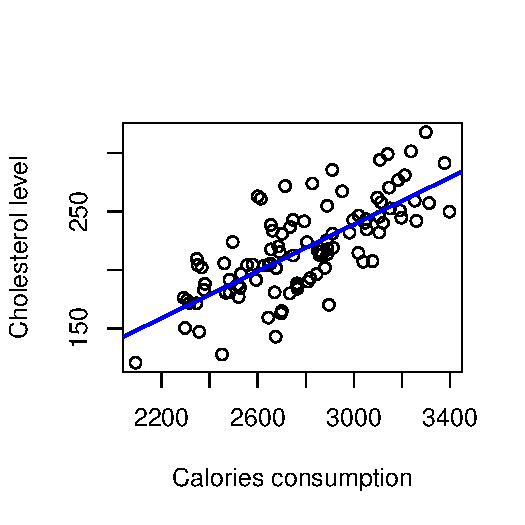
\includegraphics[width=\maxwidth]{figure/lm-1} 

\end{knitrout}
\end{frame}


\begin{frame}{Linear regression}

$$ Y = \alpha + \beta_1 X_1 + \beta_2 X_2 + \ldots + \beta_n X_n + \epsilon $$

\begin{itemize}
\item $\alpha$ correspond to the mean level of $Y$ in the population
\item $\beta_j$ indicates the change in Y when $X_j$ changes in 1 unit (after keeping the rest of $X_k$ fixed) 
\end{itemize}

\end{frame}

\begin{frame}[fragile]{Linear regression}

\textbf{Example:} Researchers are interested in knowing the factors that better explain 
air Ozone levels (variable {\tt Ozone} in data frame {\tt airquality}). They measure 
solar radiation ({\tt Solar.R}), average wind ({\tt Wind}) and temperature ({\tt Temp})
in different months (({\tt Months}) for 154 observations.

\begin{knitrout}
\definecolor{shadecolor}{rgb}{0.969, 0.969, 0.969}\color{fgcolor}\begin{kframe}
\begin{alltt}
\hlkwd{data}\hlstd{(airquality)}
\hlkwd{head}\hlstd{(airquality)}
\end{alltt}
\begin{verbatim}
##   Ozone Solar.R Wind Temp Month Day
## 1    41     190  7.4   67     5   1
## 2    36     118  8.0   72     5   2
## 3    12     149 12.6   74     5   3
## 4    18     313 11.5   62     5   4
## 5    NA      NA 14.3   56     5   5
## 6    28      NA 14.9   66     5   6
\end{verbatim}
\end{kframe}
\end{knitrout}
\end{frame}


\begin{frame}[fragile]{Linear regression}

\textbf{Simple linear regression}
\begin{knitrout}
\definecolor{shadecolor}{rgb}{0.969, 0.969, 0.969}\color{fgcolor}\begin{kframe}
\begin{alltt}
\hlstd{mod} \hlkwb{<-} \hlkwd{lm}\hlstd{(Ozone} \hlopt{~} \hlstd{Temp,} \hlkwc{data}\hlstd{=airquality)}
\hlkwd{summary}\hlstd{(mod)}
\end{alltt}
\begin{verbatim}
## 
## Call:
## lm(formula = Ozone ~ Temp, data = airquality)
## 
## Residuals:
##     Min      1Q  Median      3Q     Max 
## -40.729 -17.409  -0.587  11.306 118.271 
## 
## Coefficients:
##              Estimate Std. Error t value Pr(>|t|)    
## (Intercept) -146.9955    18.2872  -8.038 9.37e-13 ***
## Temp           2.4287     0.2331  10.418  < 2e-16 ***
## ---
## Signif. codes:  0 '***' 0.001 '**' 0.01 '*' 0.05 '.' 0.1 ' ' 1
## 
## Residual standard error: 23.71 on 114 degrees of freedom
##   (37 observations deleted due to missingness)
## Multiple R-squared:  0.4877,	Adjusted R-squared:  0.4832 
## F-statistic: 108.5 on 1 and 114 DF,  p-value: < 2.2e-16
\end{verbatim}
\end{kframe}
\end{knitrout}
\end{frame}

\begin{frame}[fragile]{Linear regression}

\textbf{Multiple linear regression}
\begin{knitrout}
\definecolor{shadecolor}{rgb}{0.969, 0.969, 0.969}\color{fgcolor}\begin{kframe}
\begin{alltt}
\hlstd{mod} \hlkwb{<-} \hlkwd{lm}\hlstd{(Ozone} \hlopt{~} \hlstd{Solar.R} \hlopt{+} \hlstd{Wind} \hlopt{+} \hlstd{Temp} \hlopt{+} \hlkwd{as.factor}\hlstd{(Month),}
          \hlkwc{data}\hlstd{=airquality)}
\hlkwd{summary}\hlstd{(mod)}
\end{alltt}
\begin{verbatim}
## 
## Call:
## lm(formula = Ozone ~ Solar.R + Wind + Temp + as.factor(Month), 
##     data = airquality)
## 
## Residuals:
##     Min      1Q  Median      3Q     Max 
## -40.344 -13.495  -3.165  10.399  92.689 
## 
## Coefficients:
##                    Estimate Std. Error t value Pr(>|t|)    
## (Intercept)       -74.23481   26.10184  -2.844  0.00537 ** 
## Solar.R             0.05222    0.02367   2.206  0.02957 *  
## Wind               -3.10872    0.66009  -4.710 7.78e-06 ***
## Temp                1.87511    0.34073   5.503 2.74e-07 ***
## as.factor(Month)6 -14.75895    9.12269  -1.618  0.10876    
## as.factor(Month)7  -8.74861    7.82906  -1.117  0.26640    
## as.factor(Month)8  -4.19654    8.14693  -0.515  0.60758    
## as.factor(Month)9 -15.96728    6.65561  -2.399  0.01823 *  
## ---
## Signif. codes:  0 '***' 0.001 '**' 0.01 '*' 0.05 '.' 0.1 ' ' 1
## 
## Residual standard error: 20.72 on 103 degrees of freedom
##   (42 observations deleted due to missingness)
## Multiple R-squared:  0.6369,	Adjusted R-squared:  0.6122 
## F-statistic: 25.81 on 7 and 103 DF,  p-value: < 2.2e-16
\end{verbatim}
\end{kframe}
\end{knitrout}
\end{frame}

\begin{frame}[fragile]{Linear regression}
\textbf{Interpretation of categorical factors}
\begin{knitrout}
\definecolor{shadecolor}{rgb}{0.969, 0.969, 0.969}\color{fgcolor}
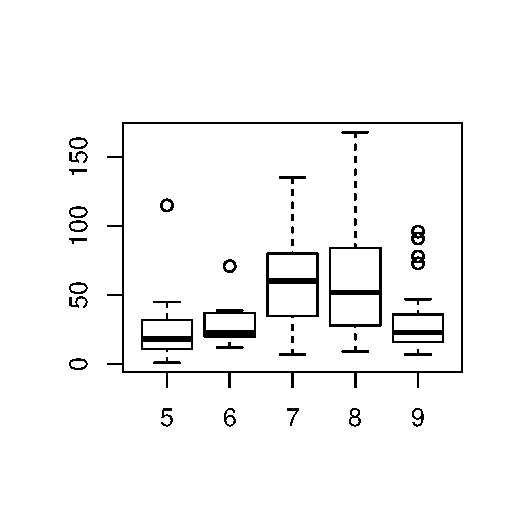
\includegraphics[width=\maxwidth]{figure/lmModF-1} 

\end{knitrout}
\end{frame}



\begin{frame}[fragile]{Linear regression}
\textbf{Model validation}
\begin{knitrout}
\definecolor{shadecolor}{rgb}{0.969, 0.969, 0.969}\color{fgcolor}\begin{kframe}
\begin{alltt}
\hlkwd{par}\hlstd{(}\hlkwc{mfrow}\hlstd{=}\hlkwd{c}\hlstd{(}\hlnum{2}\hlstd{,}\hlnum{2}\hlstd{))}
\hlkwd{plot}\hlstd{(mod)}
\end{alltt}
\end{kframe}
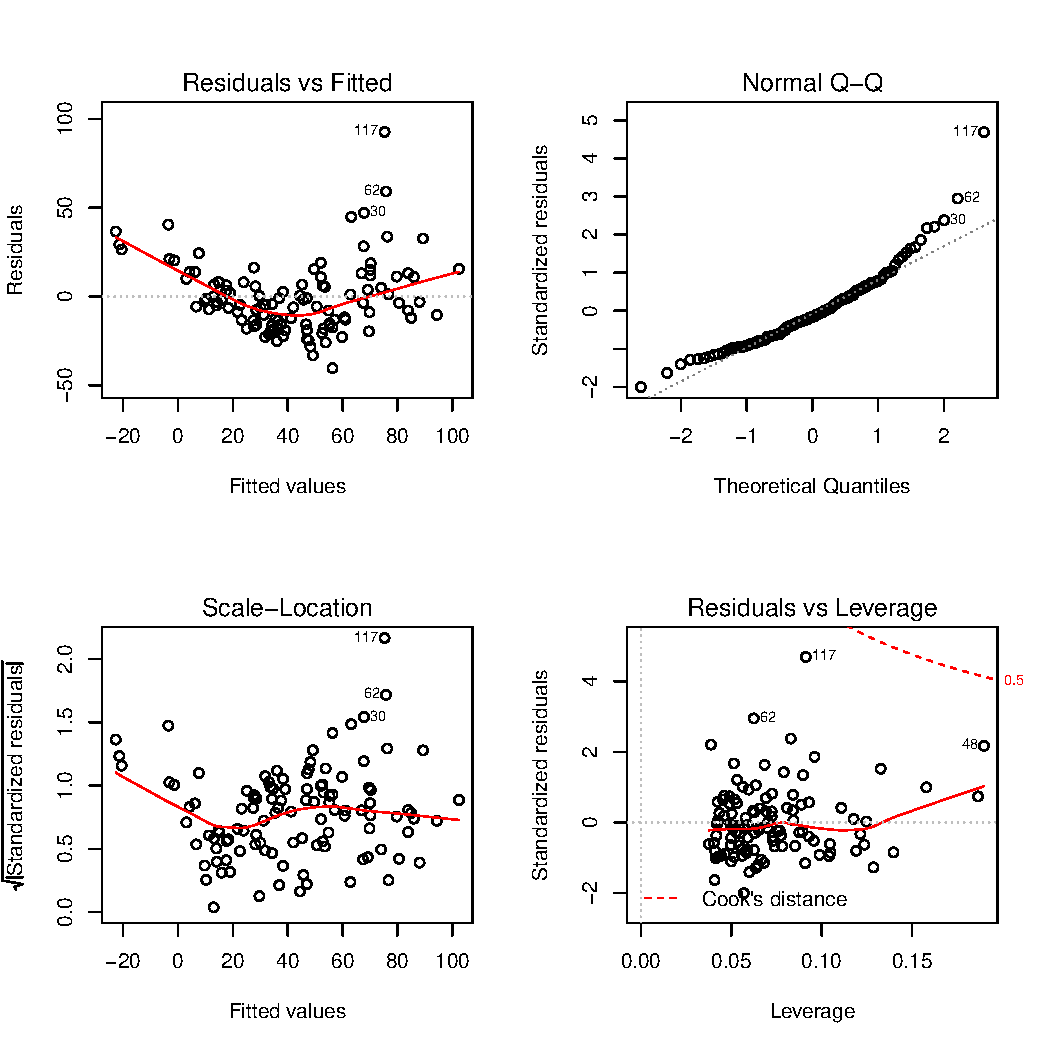
\includegraphics[width=\maxwidth]{figure/lmModVal-1} 

\end{knitrout}
\end{frame}

\begin{frame}[fragile]{Linear regression}

\begin{knitrout}
\definecolor{shadecolor}{rgb}{0.969, 0.969, 0.969}\color{fgcolor}
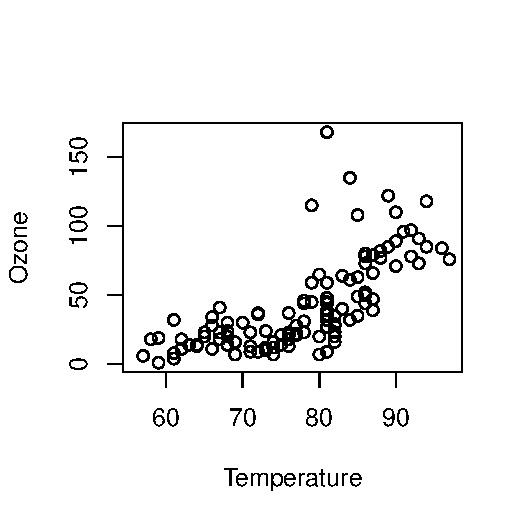
\includegraphics[width=\maxwidth]{figure/lmModPlot-1} 

\end{knitrout}
\end{frame}

\begin{frame}[fragile]{Linear regression}
\begin{knitrout}
\definecolor{shadecolor}{rgb}{0.969, 0.969, 0.969}\color{fgcolor}\begin{kframe}
\begin{alltt}
\hlkwd{require}\hlstd{(car)}
\end{alltt}


{\ttfamily\noindent\itshape\color{messagecolor}{\#\# Loading required package: car}}

{\ttfamily\noindent\itshape\color{messagecolor}{\#\# Loading required package: carData}}\begin{alltt}
\hlstd{trans} \hlkwb{<-} \hlkwd{powerTransform}\hlstd{(mod)}
\hlstd{trans}
\end{alltt}
\begin{verbatim}
## Estimated transformation parameter 
##        Y1 
## 0.2206725
\end{verbatim}
\end{kframe}
\end{knitrout}

\begin{knitrout}
\definecolor{shadecolor}{rgb}{0.969, 0.969, 0.969}\color{fgcolor}\begin{kframe}
\begin{alltt}
\hlstd{Ozone.trans} \hlkwb{<-} \hlkwd{bcPower}\hlstd{(airquality}\hlopt{$}\hlstd{Ozone,}
                       \hlkwd{coef}\hlstd{(trans,} \hlkwc{round}\hlstd{=}\hlnum{TRUE}\hlstd{))}

\hlstd{mod.trans} \hlkwb{<-} \hlkwd{lm}\hlstd{(Ozone.trans} \hlopt{~} \hlstd{Temp,} \hlkwc{data}\hlstd{=airquality)}
\end{alltt}
\end{kframe}
\end{knitrout}
\end{frame}

\begin{frame}[fragile]{Linear regression}

\begin{knitrout}
\definecolor{shadecolor}{rgb}{0.969, 0.969, 0.969}\color{fgcolor}\begin{kframe}
\begin{alltt}
\hlkwd{plot}\hlstd{(Ozone.trans} \hlopt{~} \hlstd{Temp,} \hlkwc{data}\hlstd{=airquality)}
\hlkwd{abline}\hlstd{(mod.trans,} \hlkwc{col}\hlstd{=}\hlstr{"blue"}\hlstd{)}
\end{alltt}
\end{kframe}
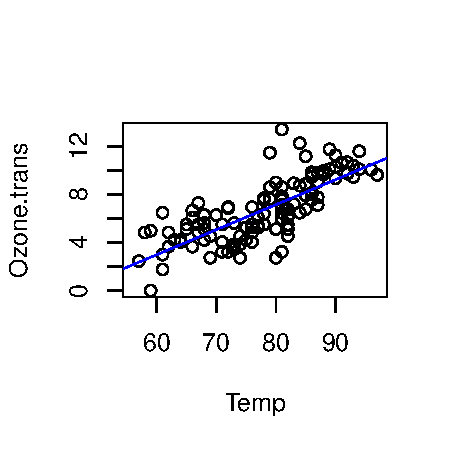
\includegraphics[width=\maxwidth]{figure/linerizationFig-1} 

\end{knitrout}
\end{frame}


\begin{frame}[fragile]{Linear regression}

Model validity can be measured by computing $R^2$

\scriptsize
\begin{knitrout}
\definecolor{shadecolor}{rgb}{0.969, 0.969, 0.969}\color{fgcolor}\begin{kframe}
\begin{alltt}
\hlkwd{summary}\hlstd{(mod)}
\end{alltt}
\begin{verbatim}
## 
## Call:
## lm(formula = Ozone ~ Temp, data = airquality)
## 
## Residuals:
##     Min      1Q  Median      3Q     Max 
## -40.729 -17.409  -0.587  11.306 118.271 
## 
## Coefficients:
##              Estimate Std. Error t value Pr(>|t|)    
## (Intercept) -146.9955    18.2872  -8.038 9.37e-13 ***
## Temp           2.4287     0.2331  10.418  < 2e-16 ***
## ---
## Signif. codes:  0 '***' 0.001 '**' 0.01 '*' 0.05 '.' 0.1 ' ' 1
## 
## Residual standard error: 23.71 on 114 degrees of freedom
##   (37 observations deleted due to missingness)
## Multiple R-squared:  0.4877,	Adjusted R-squared:  0.4832 
## F-statistic: 108.5 on 1 and 114 DF,  p-value: < 2.2e-16
\end{verbatim}
\end{kframe}
\end{knitrout}
\normalsize
\end{frame}


\begin{frame}[fragile]{Linear regression}
\scriptsize
\begin{knitrout}
\definecolor{shadecolor}{rgb}{0.969, 0.969, 0.969}\color{fgcolor}\begin{kframe}
\begin{alltt}
\hlkwd{summary}\hlstd{(mod.trans)}
\end{alltt}
\begin{verbatim}
## 
## Call:
## lm(formula = Ozone.trans ~ Temp, data = airquality)
## 
## Residuals:
##     Min      1Q  Median      3Q     Max 
## -4.4144 -1.2733  0.0883  1.1028  6.0558 
## 
## Coefficients:
##             Estimate Std. Error t value Pr(>|t|)    
## (Intercept)  -9.5085     1.3495  -7.046 1.49e-10 ***
## Temp          0.2082     0.0172  12.099  < 2e-16 ***
## ---
## Signif. codes:  0 '***' 0.001 '**' 0.01 '*' 0.05 '.' 0.1 ' ' 1
## 
## Residual standard error: 1.75 on 114 degrees of freedom
##   (37 observations deleted due to missingness)
## Multiple R-squared:  0.5622,	Adjusted R-squared:  0.5584 
## F-statistic: 146.4 on 1 and 114 DF,  p-value: < 2.2e-16
\end{verbatim}
\end{kframe}
\end{knitrout}
\normalsize
\end{frame}


\begin{frame}[fragile]{Logistic regression}

$Y$ variable is binary (case/control, relapse/non-relapse, mortality, ...). In that case, the logit
transformation guarantees linearity.

$$ \log(p(Y=1)/(1-p(Y=1))) = \alpha + \beta_1 X_1 + \ldots + \beta_k X_k $$

$\exp(\beta_k)$ can be interpreted as the odds ratio (OR) of having/developing/being $Y=1$

\end{frame}


\begin{frame}[fragile]{Logistic regression}

\textbf{Example}: Reserchers are interested in determining whether a new treatment (varible {\tt rx})
reduces mortality (variable {\tt fustat}) in patients diagnosed with ovarian cancer. 
Data are available by typing:

\begin{knitrout}
\definecolor{shadecolor}{rgb}{0.969, 0.969, 0.969}\color{fgcolor}\begin{kframe}
\begin{alltt}
\hlkwd{data}\hlstd{(ovarian,} \hlkwc{package}\hlstd{=}\hlstr{"survival"}\hlstd{)}
\hlkwd{head}\hlstd{(ovarian)}
\end{alltt}
\begin{verbatim}
##   futime fustat     age resid.ds rx ecog.ps
## 1     59      1 72.3315        2  1       1
## 2    115      1 74.4932        2  1       1
## 3    156      1 66.4658        2  1       2
## 4    421      0 53.3644        2  2       1
## 5    431      1 50.3397        2  1       1
## 6    448      0 56.4301        1  1       2
\end{verbatim}
\end{kframe}
\end{knitrout}
\end{frame}


\begin{frame}[fragile]{Logistic regression}

\scriptsize
\begin{knitrout}
\definecolor{shadecolor}{rgb}{0.969, 0.969, 0.969}\color{fgcolor}\begin{kframe}
\begin{alltt}
\hlstd{mod2} \hlkwb{<-} \hlkwd{glm}\hlstd{(fustat} \hlopt{~} \hlstd{rx,} \hlkwc{data}\hlstd{=ovarian,} \hlkwc{family}\hlstd{=}\hlstr{"binomial"}\hlstd{)}
\hlkwd{summary}\hlstd{(mod2)}
\end{alltt}
\begin{verbatim}
## 
## Call:
## glm(formula = fustat ~ rx, family = "binomial", data = ovarian)
## 
## Deviance Residuals: 
##     Min       1Q   Median       3Q      Max  
## -1.2435  -0.9854  -0.9854   1.1127   1.3824  
## 
## Coefficients:
##             Estimate Std. Error z value Pr(>|z|)
## (Intercept)   0.7783     1.2502   0.623    0.534
## rx           -0.6242     0.7966  -0.784    0.433
## 
## (Dispersion parameter for binomial family taken to be 1)
## 
##     Null deviance: 35.890  on 25  degrees of freedom
## Residual deviance: 35.268  on 24  degrees of freedom
## AIC: 39.268
## 
## Number of Fisher Scoring iterations: 4
\end{verbatim}
\end{kframe}
\end{knitrout}

\normalsize
\end{frame}


\end{document}





